\startchapter{Background}
\label{chapter:problem}

%Mathematical definition of variables
\newcommand{\timevar}{t}
\newcommand{\meas}{y}
\newcommand{\locvar}{z}
\newcommand{\est}{\hat{y}}
\newcommand{\nSampLoc}{N}
\newcommand{\nSimLoc}{n}
\newcommand{\nSampTime}{T}
\newcommand{\param}{x}
\newcommand{\conc}{u}
\newcommand{\diffCoeff}{D}
\newcommand{\advecCoeff}{\ensuremath{\alpha}}
\newcommand{\biodegCoeff}{\ensuremath{\beta}}
\newcommand{\distvar}{d}
\newcommand{\idwpow}{p}
\newcommand{\idwwin}{w}
\newcommand{\forwardFunc}{\mathcal{M}}
\newcommand{\observationFunc}{\mathcal{H}}
\newcommand{\numIterations}{K}
\newcommand{\paramComp}{X}


This chapter establishes the mathematical framework underlying the spatial interpolation problem studied in this thesis. Each method is situated within the context of soil contaminant transport and remediation. The core task is to estimate the spatial distribution of a petrochemical contaminant plume from a sparse, noise set of measurements collected across space and time. Each method considered approaches this task from a different theoretical perspective, ranging from purely geometric interpolation to physics-informed parameter estimation.

Measurements $\meas(\locvar,\timevar)$ are acquired at a spatial location $\locvar$ and time $\timevar$. The variable $\locvar$ was used since our problem is reduced to one-dimension in depth and $\locvar$ is a common notation for depth. Each evaluated method produces an estimate $\est(\locvar_o,\timevar)$ at unmeasured depths $\locvar_o$, which is compared against available ground truth via the Mean Squared Error (MSE), $(\meas(\locvar_o,\timevar) - \est(\locvar_o,\timevar))^2$, at a given time $\timevar$.  In practice, a continuous spatial ground truth is only available when working with synthetic data. For real-world datasets, leave-$n$-out cross-validation is employed as a substitute. It is also worth noting that $\timevar$ typically corresponds to the current or most recent time step, as remediators are primarily concerned with the present-day plume distribution. Within the broader spatial interpolation literature, $\meas$ is an unconventional choice of notation; however, it is adopted here because it aligns naturally with the parameter estimation and data assimilation formulations introduced later, where this notation is standard.

\section{Inverse Distance Weighting}
\label{sec:background_idw}

Inverse Distance Weighting is the simplest method evaluated in this thesis and serves as a baseline against which the more sophisticated approaches are benchmarked. It relies solely on the geometric relationship between measurement locations and the target estimation point, making no assumptions about the underlying physical process and only minimally exploiting the temporal structure of the data. Despite its simplicity, IDW provides an important reference point for understanding when temporal dynamics and physics-based constraints meaningfully improve estimation performance, and when the additional complexity of those approaches offers little advantage over a naive geometric approach.

Standard IDW computes a weighted average over all $\nSampLoc$ measurement points  at a given time $\timevar$. The weight of each measurement is relative to the inverse of the distance between the measurement depth and the target depth $\locvar_o$ raised to a user-specified power.

 \begin{equation}
 \label{eq:idw}
    \est(\locvar_o,\timevar) = 
    \frac{\sum_{i=1}^{\nSampLoc} w_i \cdot \meas(\locvar_i,\timevar)}
         {\sum_{i=1}^{\nSampLoc} w_i}, 
    \qquad w_i = \frac{1}{d(\locvar_o,\locvar_i)^p}
 \end{equation}
 
A minor modification is introduced to tailor IDW to the time-series element of this problem. Rather than using only the instantaneous measurement $\meas(\locvar_i,\timevar)$ at each location, the algorithm is supplied with the average of the most recent $\idwwin$ observations at that location. This windowed average serves to dampen measurement noise without fundamentally altering the character of the algorithm. In summary, IDW uses two hyperparameters $\idwpow$, the power of the distance relationship and $\idwwin$, the width of the temporal averaging window.






\section{Kriging}
\label{sec:background_kriging}

Kriging is a geostatistical interpolation method that shares the weighted-average structure of IDW but replaces the fixed power-law decay with an adaptive weighting scheme derived from the spatial covariance structure of the data, allowing it to capture a wider variety of spatial dependence patterns.

As with IDW, traditional Kriging treats each location independently, drawing on a single observation per site at time $\timevar$ \cite{kriging_overview}. The foundational quantity in Kriging is the semi-variance between a pair of measurement locations $\locvar_{i_1}$ and $\locvar_{i_2}$, defined as:

\begin{equation}
   \label{eq:semVar2}
   \gamma(\locvar_{i_1}, \locvar_{i_2}) 
   = \frac{1}{2} \left(\meas(\locvar_{i_1},\timevar) 
   - \meas(\locvar_{i_2},\timevar)\right)^2
\end{equation}

Computing this quantity for all pairs of measurement locations and plotting the results as a function of pairwise separation distance yields the empirical variogram, an example of which is shown in Figure~\ref{fig:kriging_semVar}.

\begin{figure}[H]
    \centering
    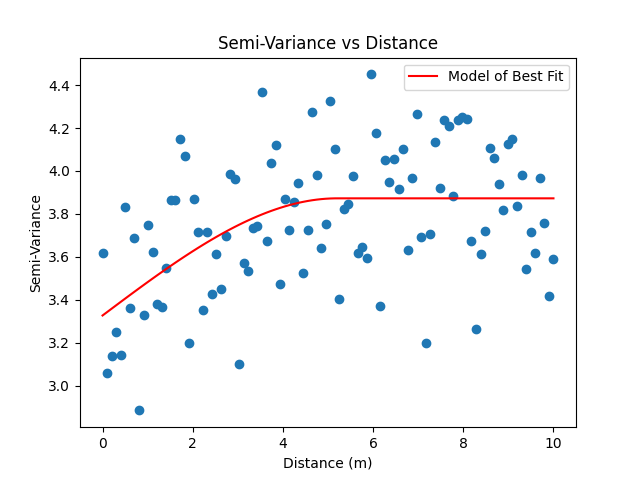
\includegraphics[height=4in]{figures/semVar.png}
    \caption{Example empirical variogram constructed from pairwise semi-variance values plotted against separation distance. Parametric model in red fit to the semi-variance values.}
    \label{fig:kriging_semVar}
\end{figure}

A parametric model is then fit to the empirical variogram. Common choices include spherical, circular, exponential, Gaussian, and linear models, each encoding a different assumption about how spatial correlation decays with distance \cite{kriging_how_to}. Model selection is typically a subjective judgment based on goodness-of-fit to the empirical data. Due to the large amounts of testing data the SciPy minimize library finds a locally optimal set of parameters for each parametric model. The fitted model is then used to evaluate the expected semi-variance at any arbitrary separation distance, including distances corresponding to unmeasured locations. These predicted semi-variances are used to construct the Kriging weights, which replace the fixed power-law weights in Equation~\ref{eq:idw} with a set of weights that minimize estimation variance subject to an unbiasedness constraint.

Two modifications are made to this standard formulation to better exploit the temporal structure of the data. The first replaces the single-snapshot semi-variance of Equation~\ref{eq:semVar2} with an average over all $\nSampTime$ time steps at which both locations have concurrent observations:

\begin{equation}
    \label{eq:semVar_more}
    \gamma(\locvar_{i_1}, \locvar_{i_2}) 
    = \frac{1}{2\nSampTime} \sum_{j_1=1}^{\nSampTime} \left(\meas(\locvar_{i_1}, \timevar_{j_1}) 
    - \meas(\locvar_{i_2}, \timevar_{j_1})\right)^2
\end{equation}

This temporal semi-variance produces a more stable empirical variogram by pooling information across time rather than relying on a single snapshot. The second modification replaces the semi-variance entirely with the Pearson correlation computed across all $\nSampTime$ concurrent observations at $\locvar_{i_1}$ and $\locvar_{i_2}$:

\begin{equation}
    \label{eq:pearsonCorr}
    \rho(\locvar_{i_1}, \locvar_{i_2})
    = \frac{\sum_{j_1=1}^{\nSampTime} 
        \left(\meas(\locvar_{i_1}, \timevar_{j_1}) - \bar{\meas}(\locvar_{i_1})\right)
        \left(\meas(\locvar_{i_2}, \timevar_{j_1}) - \bar{\meas}(\locvar_{i_2})\right)}
    {\sqrt{\sum_{j_1=1}^{\nSampTime} 
        \left(\meas(\locvar_{i_1}, \timevar_{j_1}) - \bar{\meas}(\locvar_{i_1})\right)^2}
     \sqrt{\sum_{j_1=1}^{\nSampTime} 
        \left(\meas(\locvar_{i_2}, \timevar_{j_1}) - \bar{\meas}(\locvar_{i_2})\right)^2}}
\end{equation}

Rather than measuring the magnitude of differences between locations, Pearson correlation captures the degree to which two locations co-vary over time, providing a complementary characterization of spatial dependence. Single semi-variance, temporal semi-variance, and Pearson correlation are independent dissimilarity metrics populating the empirical variogram, and their relative performance is evaluated in Section~\ref{sec:krig_tuning}.




\section{Parameter Estimation} 

4D Variational Data Assimilation (4D-Var), the Gauss-Levenberg-Marquardt algorithm (GLM), and the Iterative Ensemble Smoother (IES) share the parameter estimation framework that distinguishes them from the distance-based approaches above. Rather than interpolating directly from observed concentrations, these methods optimize a physics-based model of contaminant transport to match spatiotemporal measurements. The parameters of this forward model are estimated so that the model's simulated temporal evolution at the sensor locations matches the available measurements as closely as possible. Once the model has been adequately calibrated or a maximum number of iterations $(\numIterations)$ has been reached, the resulting spatial concentration field at the end of the simulation serves as the spatial estimate. This approach affords a significant advantage over purely geometric methods. Physical constraints such as advection, diffusion, and biodegradation are implicitly embedded in the estimate, allowing the model to extrapolate into unobserved regions of the domain in a physically consistent manner. The cost function shared by all three methods evalutes the mean squared error between the model output and the measurements across provided sensor locations and time steps:

\begin{equation}
   \label{eq:paramEst_costFunc}
   \mathcal{J} = \sum_{i=1}^{\nSampLoc}\sum_{t=1}^{\nSampTime}(\est(\locvar_i,t) - \meas(\locvar_i,t))^2
\end{equation}

\noindent
where $\nSampLoc$ is the number of sensor locations and $\nSampTime$ is the number of temporal measurements at each sensor location. The dynamical system within which these methods operate is described by a state-space model consisting of a state evolution equation, an observation equation and a smoother update equation.

\begin{equation}
   \label{eq:enkf_M}
    \hat{\paramComp}^{(k)} = \forwardFunc(\hat{\param}_{0}^{(k)}, w_\timevar), 
    \qquad w_\timevar \sim \mathcal{N}_n(0, Q) 
\end{equation}
\vspace{-1em}
\begin{equation} 
   \label{eq:enkf_H}
    \est = \observationFunc(\hat{\paramComp}^{(k)}, v_\timevar), 
    \qquad v_\timevar \sim \mathcal{N}_{m_\timevar}(0, R)
\end{equation}
\begin{equation}
    \label{eq:smoother_update}
    \hat{\param}_0^{(k+1)} \leftarrow \hat{\param}_0^{(k)} + \delta\mathcal{J}
\end{equation}

Here, $\hat{\param}_0^{(k)}$ denotes the $k^{th}$ estimate of the parameter vector and $\est$ denotes the predicted observation vector over all sensor locations and selected time steps. The operator $\forwardFunc$ is the forward model, which propagates the initial condition $\hat{\param}_0$ forward to produce the full simulated trajectory $\hat{\paramComp}$. The operator $\observationFunc$ maps this trajectory to the observation space, yielding $\est$. The terms $w_\timevar$ and $v_\timevar$ represent zero-mean Gaussian process and observation noise, with covariance matrices $Q$ and $R$, respectively. Finally, Equation \ref{eq:smoother_update} denotes the smoothing update where $\hat{\param}_0^{(k+1)}$ represents the updated parameter vector based on the method-specific update term $\delta\mathcal{J}$.

Several aspects of this formulation are worth clarifying in the context of the present problem. The observation vector $\est$ is defined over both space and time, yielding a two-dimensional array of size $(\nSampLoc\times\nSampTime)$. In practice, this is flattened into a one-dimensional vector for computational convenience. The state vector $\hat{\param}_0$ is domain-dependent: in numerical weather prediction it may represent only the physical state of the system (e.g., the concentration field $\conc$ itself), whereas in the soil contaminant setting considered here it also encompasses the physical parameters of the transport process (diffusion coefficient $\diffCoeff$, advection coefficient $\advecCoeff$, and biodegradation coefficient $\biodegCoeff$). Although these parameters do not evolve in time, they are included in the initial condition vector so that the smoother update can jointly refine both the concentration field and the underlying physical parameters.

4D-Var, GLM, and IES operate within this state-space framework, minimizing $\mathcal{J}$ by iteratively applying the smoother update in Eq.~\ref{eq:smoother_update}. Where they differ is in the strategy employed to compute the correction $\delta\mathcal{J}$ at each iteration.

Finally, all of the above is the parameter estimation process of matching the supplied spatiotemporal data $\meas$. To utilize these methods as spatial interpolation algorithms there is one final step. After either a stopping condition is met or all$\numIterations$ iterations are completed, the algorithms produce a $\est$ that matches $\meas$ as closely as possible. Alongside this is $\paramComp^\numIterations$ which is complete simulated trajectory of all simulated cells and time steps. From $paramComp^\numIterations$ we extract $\param_\nSampTime^\numIterations$ which represents the parameter vector at the time step $\nSampTime$. This vector includes the fine-grained concentration field $\conc_\nSampTime$ alongside the soil parameters and boundary conditions. The concentration field becomes the best estimate of the spatial distribution 






\subsection{4D Variational Data Assimilation (4D-Var)}
\label{sec:background_fdvar}

4D Variational Data Assimilation, commonly referred to as 4D-Var, is a deterministic optimization method that seeks to find the initial condition $\hat{\param}_0$ that minimizes the discrepancy between model predictions and observations across a defined assimilation window $[0, T]$ \cite{fdvar_og}. It has been the standard approach in operational numerical weather prediction for decades, but is less common in soil remediation practice due to its emphasis on refining initial conditions rather than stationary model parameters\cite{da_overview}.

In addition to the general cost function in Equation \ref{eq:paramEst_costFunc}, the 4D-Var cost function augments the data misfit in Equation~\ref{eq:paramEst_costFunc}. Using a regularization term that penalizes departures from a prior estimate $\param^b$ of the initial condition, weighted by the background error covariance matrix $B$:

\begin{equation}
   \label{eq:4dvar_cost}
   \mathcal{J}(\hat{\param}_0) = \frac{1}{2}(\hat{\param}_0 - \param^b)^\top 
   B^{-1}(\hat{\param}_0 - \param^b)
   + \frac{1}{2}\sum_{t=1}^{\nSampTime}
   \left(H(\hat{\param}_\nSampTime) - \meas_\timevar\right)^\top R^{-1}
   \left(H(\hat{\param}_\nSampTime) - \meas_\timevar\right)
\end{equation}

The first term encodes prior knowledge about the plausible range of parameter 
values and acts as a regularizer that prevents overfitting to the observed data. 
The second term is the observation misfit, accumulated over all assimilation 
times and weighted by the inverse of the observation error covariance $R$.

Minimizing $\mathcal{J}$ requires the gradient with respect to the initial 
condition $\nabla_{\hat{\param}_0}\mathcal{J}$, which is computed efficiently 
via the adjoint of the forward model $M$. The adjoint equations propagate the 
observation residuals backward through time, yielding the exact gradient of the 
cost function at a computational cost comparable to a single forward model 
integration, regardless of the dimension of $\hat{\param}_0$. This property 
makes 4D-Var well suited to high-dimensional problems\cite{fdvar_details}.

Given the gradient, the smoother update in Equation~\ref{eq:smoother_update} is 
applied using a gradient-based optimizer such as L-BFGS or a truncated Newton 
method, where the correction $\delta\mathcal{J}$ is computed from 
$\nabla_{\hat{\param}_0}\mathcal{J}$ at each iteration. Iteration proceeds until 
the gradient norm falls below a specified tolerance or a maximum number of 
forward model evaluations is reached. In the present application, $\hat{\param}_0$ 
contains the initial concentration field $\conc$ alongside the physical transport 
parameters $\diffCoeff$, $\advecCoeff$, and $\biodegCoeff$; all are updated 
jointly through the adjoint-based optimization.









\subsection{Gauss-Levenberg-Marquardt (GLM)}
\label{sec:background_glm}

The Gauss-Levenberg-Marquardt (GLM) algorithm, as implemented in the PEST software suite \cite{pestManual}, is a gradient-based nonlinear least-squares method. It belongs to the family of trust-region methods and can be understood as a regularized form of the classical Gauss-Newton algorithm. GLM has been widely applied to groundwater model calibration and contaminant transport inverse problems, where it remains a practical workhorse owing to its relative computational efficiency and well-understood convergence properties.

At each iteration, GLM linearizes the forward model $M$ around the current estimate of the initial condition $\hat{\param}_0^{(k)}$ by computing the Jacobian matrix:

\begin{equation}
   \label{eq:jacobian}
   J_{ij} = \frac{\partial \est(\locvar_i, t)}{\partial \hat{\param}_{0,j}}
   \Bigg|_{\hat{\param}_0^{(k)}}
\end{equation}

where the $(i,j)$ entry gives the sensitivity of the model output at depth 
$\locvar_i$ and time $t$ to a perturbation in the $j$-th component of 
$\hat{\param}_0$. This Jacobian is estimated by finite differences, 
requiring one forward model run per parameter.

The smoother update in Equation~\ref{eq:smoother_update} is then applied with 
the correction $\delta\mathcal{J}$ computed as:

\begin{equation}
   \label{eq:glm_update}
   \delta\mathcal{J} = \left(J^\top R^{-1} J + \lambda I\right)^{-1} J^\top 
   R^{-1}\left(\meas - \est(\hat{\param}_0^{(k)})\right)
\end{equation}

The scalar $\lambda \geq 0$ is the Marquardt parameter, which controls the 
interpolation between a pure Gauss-Newton step ($\lambda = 0$, fast convergence 
near the optimum) and a steepest-descent step ($\lambda \to \infty$, robust far 
from the optimum). PEST adapts $\lambda$ automatically across iterations using a 
line-search heuristic: $\lambda$ is increased when $\mathcal{J}$ fails to 
decrease, and reduced when sufficient progress is made.

PEST also supports Tikhonov regularization, which augments $\mathcal{J}$ with a 
term penalizing parameter complexity --- for instance, penalizing departures from 
spatial smoothness or from physically plausible prior values. This regularization 
is particularly valuable in the present problem, where the number of parameters 
(transport coefficients together with the spatial discretization of $\conc$) may 
be large relative to the number of observations. Iteration terminates when the 
relative change in $\mathcal{J}$ falls below a threshold or the maximum number 
of forward model runs is exhausted.











where the $(i,j)$ entry gives the sensitivity of the model output at depth $\locvar_i$ and time $t$ to a perturbation in the $j$-th parameter. In PEST, this Jacobian is estimated by finite differences, requiring one forward model run per parameter.

Given the Jacobian, the parameter update is computed as:

\begin{equation}
   \label{eq:glm_update}
   \param^{(k+1)} = \param^{(k)} 
   + \left(J^\top R^{-1} J + \lambda I\right)^{-1} J^\top R^{-1}
   \left(\meas - \est(\param^{(k)})\right)
\end{equation}

The scalar $\lambda \geq 0$ is the Marquardt parameter, which controls the interpolation between a pure Gauss-Newton step ($\lambda = 0$, fast convergence near the optimum) and a steepest-descent step ($\lambda \to \infty$, robust far from the optimum). PEST adapts $\lambda$ automatically across iterations using a line-search heuristic: $\lambda$ is increased when the cost function fails to decrease, and reduced when sufficient progress is made.

PEST also supports Tikhonov regularization, which augments the cost function with a term penalizing parameter complexity — for instance, penalizing departures from spatial smoothness or from physically plausible prior values. This regularization is particularly valuable in the present problem, where the number of parameters (transport coefficients together with the spatial discretization of $\conc$) may be large relative to the number of observations. Iteration terminates when the relative change in the cost function falls below a threshold or the maximum number of forward model runs is exhausted.

\subsection{PEST-IES}
\label{sec:background_ies}

The Iterative Ensemble Smoother (IES), also implemented within the PEST++ software framework \cite{pestIES}, takes a fundamentally different approach from both 4D-Var and GLM by representing uncertainty in the parameter vector through an ensemble of candidate solutions rather than seeking a single point estimate. This ensemble-based perspective is closely related to the Ensemble Kalman Filter (EnKF) and its smoothing variants, but is formulated as an iterative batch smoother that assimilates all observations simultaneously rather than sequentially.

An ensemble of $N_e$ parameter realizations $\{\param^{(j)}_0\}_{j=1}^{N_e}$ is drawn from the prior distribution $\mathcal{N}(\param^b, B)$, where $\param^b$ is the prior mean and $B$ is the prior covariance. Each realization is propagated through the forward model $M$ to produce a corresponding ensemble of simulated observations:

\begin{equation}
   \label{eq:ies_ensemble}
   \est^{(j)}_\timevar = H(M(\param^{(j)}_{\timevar-1})), 
   \qquad j = 1, \ldots, N_e
\end{equation}

The ensemble is then updated using a form of the ensemble Kalman update, in which the empirical cross-covariance between the parameter ensemble and the simulated observation ensemble is used in place of the exact Jacobian:

\begin{equation}
   \label{eq:ies_update}
   \param^{(j)} \leftarrow \param^{(j)} 
   + C_{\param \est}\left(C_{\est \est} + R\right)^{-1}
   \left(\meas^{(j)} - \est^{(j)}\right)
\end{equation}

where $C_{\param \est}$ is the ensemble cross-covariance between parameters and simulated observations, $C_{\est \est}$ is the ensemble covariance of the simulated observations, and $\meas^{(j)}$ is a perturbed observation vector drawn from $\mathcal{N}(\meas, R)$ to account for observation uncertainty. Unlike the standard EnKF, PEST-IES applies this update iteratively, re-running the forward model after each update step and recalculating the ensemble covariances. This iteration corrects for the linearization error inherent in the single-step Kalman update and allows the ensemble to converge toward the posterior distribution even in the presence of moderate nonlinearity.

A key practical advantage of PEST-IES over GLM is that it does not require explicit computation of a Jacobian matrix; the ensemble covariances implicitly provide the sensitivity information needed for the update. This makes it particularly attractive for high-dimensional problems where finite-difference Jacobian estimation would demand a prohibitive number of forward model evaluations. Furthermore, the ensemble representation naturally quantifies parametric uncertainty: the spread of the posterior ensemble directly reflects the identifiability of the parameters given the available observations, providing valuable information for decision-making in the remediation context.